\PassOptionsToPackage{unicode=true}{hyperref} % options for packages loaded elsewhere
\PassOptionsToPackage{hyphens}{url}
%
\documentclass[ignorenonframetext,]{beamer}
\usepackage{pgfpages}
\setbeamertemplate{caption}[numbered]
\setbeamertemplate{caption label separator}{: }
\setbeamercolor{caption name}{fg=normal text.fg}
\beamertemplatenavigationsymbolsempty
% Prevent slide breaks in the middle of a paragraph:
\widowpenalties 1 10000
\raggedbottom
\setbeamertemplate{part page}{
\centering
\begin{beamercolorbox}[sep=16pt,center]{part title}
  \usebeamerfont{part title}\insertpart\par
\end{beamercolorbox}
}
\setbeamertemplate{section page}{
\centering
\begin{beamercolorbox}[sep=12pt,center]{part title}
  \usebeamerfont{section title}\insertsection\par
\end{beamercolorbox}
}
\setbeamertemplate{subsection page}{
\centering
\begin{beamercolorbox}[sep=8pt,center]{part title}
  \usebeamerfont{subsection title}\insertsubsection\par
\end{beamercolorbox}
}
\AtBeginPart{
  \frame{\partpage}
}
\AtBeginSection{
  \ifbibliography
  \else
    \frame{\sectionpage}
  \fi
}
\AtBeginSubsection{
  \frame{\subsectionpage}
}
\usepackage{lmodern}
\usepackage{amssymb,amsmath}
\usepackage{ifxetex,ifluatex}
\usepackage{fixltx2e} % provides \textsubscript
\ifnum 0\ifxetex 1\fi\ifluatex 1\fi=0 % if pdftex
  \usepackage[T1]{fontenc}
  \usepackage[utf8]{inputenc}
  \usepackage{textcomp} % provides euro and other symbols
\else % if luatex or xelatex
  \usepackage{unicode-math}
  \defaultfontfeatures{Ligatures=TeX,Scale=MatchLowercase}
\fi
% use upquote if available, for straight quotes in verbatim environments
\IfFileExists{upquote.sty}{\usepackage{upquote}}{}
% use microtype if available
\IfFileExists{microtype.sty}{%
\usepackage[]{microtype}
\UseMicrotypeSet[protrusion]{basicmath} % disable protrusion for tt fonts
}{}
\IfFileExists{parskip.sty}{%
\usepackage{parskip}
}{% else
\setlength{\parindent}{0pt}
\setlength{\parskip}{6pt plus 2pt minus 1pt}
}
\usepackage{hyperref}
\hypersetup{
            pdftitle={Principal Component Analysis: An Introduction with Examples in R},
            pdfauthor={Salvatore A. Sidoti},
            pdfborder={0 0 0},
            breaklinks=true}
\urlstyle{same}  % don't use monospace font for urls
\newif\ifbibliography
\usepackage{color}
\usepackage{fancyvrb}
\newcommand{\VerbBar}{|}
\newcommand{\VERB}{\Verb[commandchars=\\\{\}]}
\DefineVerbatimEnvironment{Highlighting}{Verbatim}{commandchars=\\\{\}}
% Add ',fontsize=\small' for more characters per line
\usepackage{framed}
\definecolor{shadecolor}{RGB}{248,248,248}
\newenvironment{Shaded}{\begin{snugshade}}{\end{snugshade}}
\newcommand{\AlertTok}[1]{\textcolor[rgb]{0.94,0.16,0.16}{#1}}
\newcommand{\AnnotationTok}[1]{\textcolor[rgb]{0.56,0.35,0.01}{\textbf{\textit{#1}}}}
\newcommand{\AttributeTok}[1]{\textcolor[rgb]{0.77,0.63,0.00}{#1}}
\newcommand{\BaseNTok}[1]{\textcolor[rgb]{0.00,0.00,0.81}{#1}}
\newcommand{\BuiltInTok}[1]{#1}
\newcommand{\CharTok}[1]{\textcolor[rgb]{0.31,0.60,0.02}{#1}}
\newcommand{\CommentTok}[1]{\textcolor[rgb]{0.56,0.35,0.01}{\textit{#1}}}
\newcommand{\CommentVarTok}[1]{\textcolor[rgb]{0.56,0.35,0.01}{\textbf{\textit{#1}}}}
\newcommand{\ConstantTok}[1]{\textcolor[rgb]{0.00,0.00,0.00}{#1}}
\newcommand{\ControlFlowTok}[1]{\textcolor[rgb]{0.13,0.29,0.53}{\textbf{#1}}}
\newcommand{\DataTypeTok}[1]{\textcolor[rgb]{0.13,0.29,0.53}{#1}}
\newcommand{\DecValTok}[1]{\textcolor[rgb]{0.00,0.00,0.81}{#1}}
\newcommand{\DocumentationTok}[1]{\textcolor[rgb]{0.56,0.35,0.01}{\textbf{\textit{#1}}}}
\newcommand{\ErrorTok}[1]{\textcolor[rgb]{0.64,0.00,0.00}{\textbf{#1}}}
\newcommand{\ExtensionTok}[1]{#1}
\newcommand{\FloatTok}[1]{\textcolor[rgb]{0.00,0.00,0.81}{#1}}
\newcommand{\FunctionTok}[1]{\textcolor[rgb]{0.00,0.00,0.00}{#1}}
\newcommand{\ImportTok}[1]{#1}
\newcommand{\InformationTok}[1]{\textcolor[rgb]{0.56,0.35,0.01}{\textbf{\textit{#1}}}}
\newcommand{\KeywordTok}[1]{\textcolor[rgb]{0.13,0.29,0.53}{\textbf{#1}}}
\newcommand{\NormalTok}[1]{#1}
\newcommand{\OperatorTok}[1]{\textcolor[rgb]{0.81,0.36,0.00}{\textbf{#1}}}
\newcommand{\OtherTok}[1]{\textcolor[rgb]{0.56,0.35,0.01}{#1}}
\newcommand{\PreprocessorTok}[1]{\textcolor[rgb]{0.56,0.35,0.01}{\textit{#1}}}
\newcommand{\RegionMarkerTok}[1]{#1}
\newcommand{\SpecialCharTok}[1]{\textcolor[rgb]{0.00,0.00,0.00}{#1}}
\newcommand{\SpecialStringTok}[1]{\textcolor[rgb]{0.31,0.60,0.02}{#1}}
\newcommand{\StringTok}[1]{\textcolor[rgb]{0.31,0.60,0.02}{#1}}
\newcommand{\VariableTok}[1]{\textcolor[rgb]{0.00,0.00,0.00}{#1}}
\newcommand{\VerbatimStringTok}[1]{\textcolor[rgb]{0.31,0.60,0.02}{#1}}
\newcommand{\WarningTok}[1]{\textcolor[rgb]{0.56,0.35,0.01}{\textbf{\textit{#1}}}}
\setlength{\emergencystretch}{3em}  % prevent overfull lines
\providecommand{\tightlist}{%
  \setlength{\itemsep}{0pt}\setlength{\parskip}{0pt}}
\setcounter{secnumdepth}{0}

% set default figure placement to htbp
\makeatletter
\def\fps@figure{htbp}
\makeatother


\title{Principal Component Analysis: An Introduction with Examples in R}
\author{Salvatore A. Sidoti}
\date{2019-02-14}

\begin{document}
\frame{\titlepage}

\begin{frame}

\begin{block}{PCA}

\begin{itemize}
\tightlist
\item
  Principle component analysis distributes the variation in a
  multivariate dataset across \emph{components}.
\item
  Visualize patterns that would not be apparent
\item
  Linear algebra is at the heart of the PCA
\item
  This discussion will be light on mathematical theory
\end{itemize}

\end{block}

\end{frame}

\begin{frame}{Accomplishing the PCA \emph{Manually}}
\protect\hypertarget{accomplishing-the-pca-manually}{}

\begin{block}{Accomplishing the PCA \emph{Manually}}

\begin{itemize}
\tightlist
\item
  Goal for the \emph{manual} PCA
\item
  Become acquainted with the terminology and concepts in PCA
\item
  Better prepared to defend your analysis
\end{itemize}

\end{block}

\end{frame}

\begin{frame}{Motivating Example - Wolf Spider Morphometrics}
\protect\hypertarget{motivating-example---wolf-spider-morphometrics}{}

\end{frame}

\begin{frame}{}
\protect\hypertarget{section}{}

\begin{center}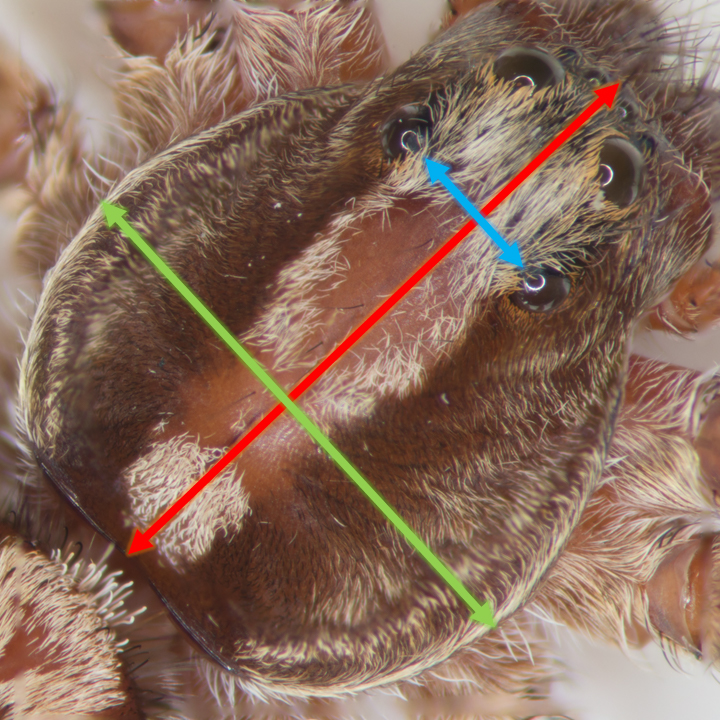
\includegraphics[width=10in]{morpho} \end{center}

\begin{block}{Descriptive Statistics}

\begingroup\fontsize{30}{32}\selectfont

\begin{tabular}{>{\bfseries}l|>{\raggedleft\arraybackslash}p{3em}|>{\raggedleft\arraybackslash}p{3em}|>{\raggedleft\arraybackslash}p{3em}|>{\raggedleft\arraybackslash}p{3em}}
\hline
\begingroup\fontsize{30}{32}\selectfont  \endgroup & \begingroup\fontsize{30}{32}\selectfont interoc\endgroup & \begingroup\fontsize{30}{32}\selectfont cwidth\endgroup & \begingroup\fontsize{30}{32}\selectfont clength\endgroup & \begingroup\fontsize{30}{32}\selectfont T.weight\endgroup\\
\hline
median & 0.798 & 2.975 & 3.706 & 1.740\\
\hline
mean & 0.799 & 2.991 & 3.691 & 1.742\\
\hline
SE.mean & 0.005 & 0.020 & 0.020 & 0.004\\
\hline
CI.mean.0.95 & 0.011 & 0.039 & 0.039 & 0.008\\
\hline
var & 0.002 & 0.028 & 0.028 & 0.001\\
\hline
std.dev & 0.046 & 0.166 & 0.167 & 0.033\\
\hline
coef.var & 0.058 & 0.055 & 0.045 & 0.019\\
\hline
\end{tabular}
\endgroup{}

\end{block}

\end{frame}

\begin{frame}{}
\protect\hypertarget{section-1}{}

\begin{center}\includegraphics[width=1\linewidth]{pca-morpho-presentation_files/figure-beamer/unnamed-chunk-4-1} \end{center}

\end{frame}

\begin{frame}{Covariance or Correlation?}
\protect\hypertarget{covariance-or-correlation}{}

\begin{block}{Covariance or Correlation?}

\begin{itemize}
\tightlist
\item
  Are the metrics in our dataset are \emph{like} or \emph{mixed}?
\item
  Like: covariance matrix with mean-centering
\item
  Mixed: correlation matrix with unit variance
\item
  Becomes essential when using the built-in PCA functions in R
\end{itemize}

\end{block}

\end{frame}

\begin{frame}[fragile]{Find the Eigenvalues \& Eigenvectors}
\protect\hypertarget{find-the-eigenvalues-eigenvectors}{}

\begin{block}{Calculating Eigenvectors}

\begin{Shaded}
\begin{Highlighting}[]
\NormalTok{standardize <-}\StringTok{ }\ControlFlowTok{function}\NormalTok{(x) \{(x }\OperatorTok{-}\StringTok{ }\KeywordTok{mean}\NormalTok{(x))}\OperatorTok{/}\KeywordTok{sd}\NormalTok{(x)\}}

\CommentTok{# Eliminate factor variables & untransformed weights}
\NormalTok{my.scaled.data <-}\StringTok{ }\KeywordTok{as.data.frame}\NormalTok{(}\KeywordTok{apply}\NormalTok{(morpho, }\DecValTok{2}\NormalTok{, standardize))}

\CommentTok{# Calculate correlation matrix}
\NormalTok{my.cor <-}\StringTok{ }\KeywordTok{cor}\NormalTok{(my.scaled.data)}

\CommentTok{# Save the eigenvalues of the correllation matrix}
\NormalTok{my.eigen <-}\StringTok{ }\KeywordTok{eigen}\NormalTok{(my.cor)}

\CommentTok{# Rename matrix rows and columns for easier interpretation}
\KeywordTok{rownames}\NormalTok{(my.eigen}\OperatorTok{$}\NormalTok{vectors) <-}\StringTok{ }\KeywordTok{c}\NormalTok{(}\StringTok{"interoc"}\NormalTok{, }\StringTok{"cwidth"}\NormalTok{,}
                                \StringTok{"clength"}\NormalTok{, }\StringTok{"T.weight"}\NormalTok{)}
\KeywordTok{colnames}\NormalTok{(my.eigen}\OperatorTok{$}\NormalTok{vectors) <-}\StringTok{ }\KeywordTok{c}\NormalTok{(}\StringTok{"PC1"}\NormalTok{, }\StringTok{"PC2"}\NormalTok{, }\StringTok{"PC3"}\NormalTok{, }\StringTok{"PC4"}\NormalTok{)}
\end{Highlighting}
\end{Shaded}

\end{block}

\begin{block}{Calculating Eigenvectors}

\begin{table}[H]
\centering\begingroup\fontsize{38}{40}\selectfont

\begin{tabular}{>{\bfseries}l|>{\raggedleft\arraybackslash}p{4em}|>{\raggedleft\arraybackslash}p{4em}|>{\raggedleft\arraybackslash}p{4em}|>{\raggedleft\arraybackslash}p{4em}}
\hline
\begingroup\fontsize{38}{40}\selectfont  \endgroup & \begingroup\fontsize{38}{40}\selectfont PC1\endgroup & \begingroup\fontsize{38}{40}\selectfont PC2\endgroup & \begingroup\fontsize{38}{40}\selectfont PC3\endgroup & \begingroup\fontsize{38}{40}\selectfont PC4\endgroup\\
\hline
interoc & -0.4973 & -0.2504 & 0.8251 & -0.0960\\
\hline
cwidth & -0.5319 & -0.3465 & -0.4948 & -0.5935\\
\hline
clength & -0.5760 & -0.0463 & -0.2716 & 0.7696\\
\hline
T.weight & -0.3716 & 0.9028 & 0.0250 & -0.2150\\
\hline
\end{tabular}
\endgroup{}
\end{table}

\end{block}

\begin{block}{Calculating Eigenvalues}

\begin{table}[H]
\centering\begingroup\fontsize{38}{40}\selectfont

\begin{tabular}{>{\bfseries}l|>{\raggedleft\arraybackslash}p{4em}}
\hline
\begingroup\fontsize{38}{40}\selectfont PC\endgroup & \begingroup\fontsize{38}{40}\selectfont eigenvalues\endgroup\\
\hline
PC1 & 2.7104\\
\hline
PC2 & 0.7608\\
\hline
PC3 & 0.4128\\
\hline
PC4 & 0.1160\\
\hline
\end{tabular}
\endgroup{}
\end{table}

\end{block}

\begin{block}{Calculating Eigenvalues}

Sum of the eigenvalues = total variance of the scaled data

\begin{Shaded}
\begin{Highlighting}[]
\KeywordTok{sum}\NormalTok{(my.eigen}\OperatorTok{$}\NormalTok{values)}
\end{Highlighting}
\end{Shaded}

\begin{verbatim}
## [1] 4
\end{verbatim}

\begin{Shaded}
\begin{Highlighting}[]
\KeywordTok{sum}\NormalTok{(}
  \KeywordTok{var}\NormalTok{(my.scaled.data[,}\DecValTok{1}\NormalTok{]),}
  \KeywordTok{var}\NormalTok{(my.scaled.data[,}\DecValTok{2}\NormalTok{]),}
  \KeywordTok{var}\NormalTok{(my.scaled.data[,}\DecValTok{3}\NormalTok{]),}
  \KeywordTok{var}\NormalTok{(my.scaled.data[,}\DecValTok{4}\NormalTok{]))}
\end{Highlighting}
\end{Shaded}

\begin{verbatim}
## [1] 4
\end{verbatim}

\end{block}

\end{frame}

\begin{frame}[fragile]{Amount of Variation Captured by the PCs}
\protect\hypertarget{amount-of-variation-captured-by-the-pcs}{}

\begin{block}{Variation Captured by the PCs}

\begin{Shaded}
\begin{Highlighting}[]
\NormalTok{pc1.var <-}\StringTok{ }\DecValTok{100}\OperatorTok{*}\KeywordTok{round}\NormalTok{(my.eigen}\OperatorTok{$}\NormalTok{values[}\DecValTok{1}\NormalTok{]}\OperatorTok{/}
\StringTok{                       }\KeywordTok{sum}\NormalTok{(my.eigen}\OperatorTok{$}\NormalTok{values), }\DataTypeTok{digits =} \DecValTok{3}\NormalTok{)}
\NormalTok{pc2.var <-}\StringTok{ }\DecValTok{100}\OperatorTok{*}\KeywordTok{round}\NormalTok{(my.eigen}\OperatorTok{$}\NormalTok{values[}\DecValTok{2}\NormalTok{]}\OperatorTok{/}
\StringTok{                       }\KeywordTok{sum}\NormalTok{(my.eigen}\OperatorTok{$}\NormalTok{values), }\DataTypeTok{digits =} \DecValTok{3}\NormalTok{)}
\NormalTok{pc3.var <-}\StringTok{ }\DecValTok{100}\OperatorTok{*}\KeywordTok{round}\NormalTok{(my.eigen}\OperatorTok{$}\NormalTok{values[}\DecValTok{3}\NormalTok{]}\OperatorTok{/}
\StringTok{                       }\KeywordTok{sum}\NormalTok{(my.eigen}\OperatorTok{$}\NormalTok{values), }\DataTypeTok{digits =} \DecValTok{3}\NormalTok{)}
\NormalTok{pc4.var <-}\StringTok{ }\DecValTok{100}\OperatorTok{*}\KeywordTok{round}\NormalTok{(my.eigen}\OperatorTok{$}\NormalTok{values[}\DecValTok{4}\NormalTok{]}\OperatorTok{/}
\StringTok{                       }\KeywordTok{sum}\NormalTok{(my.eigen}\OperatorTok{$}\NormalTok{values), }\DataTypeTok{digits =} \DecValTok{3}\NormalTok{)}

\NormalTok{pc <-}\StringTok{ }\KeywordTok{data.frame}\NormalTok{(}\DataTypeTok{PC =} \KeywordTok{c}\NormalTok{(}\StringTok{"PC1"}\NormalTok{, }\StringTok{"PC2"}\NormalTok{, }\StringTok{"PC3"}\NormalTok{, }\StringTok{"PC4"}\NormalTok{),}
                 \DataTypeTok{Percentage =} \KeywordTok{c}\NormalTok{(pc1.var, pc2.var,}
\NormalTok{                                pc3.var, pc4.var))}
\end{Highlighting}
\end{Shaded}

\end{block}

\begin{block}{Variation Captured by the PCs}

\begin{table}[H]
\centering\begingroup\fontsize{38}{40}\selectfont

\begin{tabular}{>{\bfseries}l|r}
\hline
\begingroup\fontsize{38}{40}\selectfont PC\endgroup & \begingroup\fontsize{38}{40}\selectfont Percentage\endgroup\\
\hline
PC1 & 67.8\\
\hline
PC2 & 19.0\\
\hline
PC3 & 10.3\\
\hline
PC4 & 2.9\\
\hline
\end{tabular}
\endgroup{}
\end{table}

\end{block}

\begin{block}{Variation Captured by the PCs}

The total variation should sum to \textasciitilde{}100\% depending on
rounding error:

\begin{verbatim}
## [1] 100
\end{verbatim}

\end{block}

\end{frame}

\begin{frame}[fragile]{What are PCA ``scores''?}
\protect\hypertarget{what-are-pca-scores}{}

\begin{block}{What are PCA ``scores''?}

\begin{itemize}
\tightlist
\item
  Express the loadings and scaled data as matrices, then multiply them
  together
\item
  The result is a new matrix which expresses the data in terms of the
  PCs
\item
  These are the PCA \emph{scores}
\end{itemize}

\end{block}

\begin{block}{What are PCA ``scores''?}

\begin{Shaded}
\begin{Highlighting}[]
\NormalTok{loadings <-}\StringTok{ }\NormalTok{my.eigen}\OperatorTok{$}\NormalTok{vectors}
\NormalTok{my.scaled.matrix <-}\StringTok{ }\KeywordTok{as.matrix}\NormalTok{(my.scaled.data)}
\CommentTok{# the function %*% is matrix multiplication}
\NormalTok{scores <-}\StringTok{ }\NormalTok{my.scaled.matrix }\OperatorTok\StringTok{ }\NormalTok{loadings}
\NormalTok{sd <-}\StringTok{ }\KeywordTok{sqrt}\NormalTok{(my.eigen}\OperatorTok{$}\NormalTok{values)}
\KeywordTok{rownames}\NormalTok{(loadings) <-}\StringTok{ }\KeywordTok{colnames}\NormalTok{(my.scaled.data)}
\end{Highlighting}
\end{Shaded}

\end{block}

\begin{block}{What are PCA ``scores''?}

\begin{table}[H]
\centering\begingroup\fontsize{38}{40}\selectfont

\begin{tabular}{>{\raggedleft\arraybackslash}p{4em}|>{\raggedleft\arraybackslash}p{4em}|>{\raggedleft\arraybackslash}p{4em}|>{\raggedleft\arraybackslash}p{4em}}
\hline
\begingroup\fontsize{38}{40}\selectfont PC1\endgroup & \begingroup\fontsize{38}{40}\selectfont PC2\endgroup & \begingroup\fontsize{38}{40}\selectfont PC3\endgroup & \begingroup\fontsize{38}{40}\selectfont PC4\endgroup\\
\hline
-2.2600 & 0.4796 & 0.1963 & -0.0511\\
\hline
-1.2141 & 1.0328 & 0.0185 & 0.0859\\
\hline
-2.9230 & 0.7367 & -0.3902 & 0.5873\\
\hline
-1.0990 & 1.0164 & 0.0283 & 0.0654\\
\hline
-0.5060 & 1.8150 & 0.8230 & 0.6192\\
\hline
-0.3074 & 0.8778 & 0.0583 & -0.0498\\
\hline
\end{tabular}
\endgroup{}
\end{table}

\end{block}

\end{frame}

\begin{frame}[fragile]{PCA with Native R Functions}
\protect\hypertarget{pca-with-native-r-functions}{}

\begin{block}{PCA with Native R Functions}

The function \texttt{prcomp} is the primary tool for PCA in base R

\begin{Shaded}
\begin{Highlighting}[]
\NormalTok{pca_morpho <-}\StringTok{ }\KeywordTok{prcomp}\NormalTok{(morpho, }\DataTypeTok{center =} \OtherTok{TRUE}\NormalTok{, }\DataTypeTok{scale. =} \OtherTok{TRUE}\NormalTok{)}

\CommentTok{# Show the variables in the class "prcomp"}
\KeywordTok{ls}\NormalTok{(pca_morpho)}
\end{Highlighting}
\end{Shaded}

\begin{verbatim}
## [1] "center"   "rotation" "scale"    "sdev"     "x"
\end{verbatim}

\end{block}

\begin{block}{Summary output of the PCA}

\begin{Shaded}
\begin{Highlighting}[]
\NormalTok{pca_summary <-}\StringTok{ }\KeywordTok{summary}\NormalTok{(pca_morpho)}\OperatorTok{$}\NormalTok{importance }\OperatorTok
\StringTok{  }\KeywordTok{as.data.frame}\NormalTok{() }\OperatorTok
\StringTok{  }\KeywordTok{round}\NormalTok{(., }\DataTypeTok{digits =} \DecValTok{3}\NormalTok{)}
\end{Highlighting}
\end{Shaded}

\end{block}

\begin{block}{Summary output of the PCA}

\begin{table}[H]
\centering\begingroup\fontsize{35}{37}\selectfont

\begin{tabular}{>{\raggedright\arraybackslash}p{12em}|>{\raggedleft\arraybackslash}p{3em}|>{\raggedleft\arraybackslash}p{3em}|>{\raggedleft\arraybackslash}p{3em}|r}
\hline
\begingroup\fontsize{35}{37}\selectfont  \endgroup & \begingroup\fontsize{35}{37}\selectfont PC1\endgroup & \begingroup\fontsize{35}{37}\selectfont PC2\endgroup & \begingroup\fontsize{35}{37}\selectfont PC3\endgroup & \begingroup\fontsize{35}{37}\selectfont PC4\endgroup\\
\hline
Standard deviation & 1.646 & 0.872 & 0.642 & 0.341\\
\hline
Proportion of Variance & 0.678 & 0.190 & 0.103 & 0.029\\
\hline
Cumulative Proportion & 0.678 & 0.868 & 0.971 & 1.000\\
\hline
\end{tabular}
\endgroup{}
\end{table}

\end{block}

\begin{block}{Orthogonality of PCs}

\begin{center}\includegraphics[width=1\linewidth]{pca-morpho-presentation_files/figure-beamer/unnamed-chunk-17-1} \end{center}

\end{block}

\begin{block}{Biplot}

\begin{center}\includegraphics[width=1\linewidth]{pca-morpho-presentation_files/figure-beamer/unnamed-chunk-18-1} \end{center}

\end{block}

\end{frame}

\begin{frame}[fragile]{How many PCs explain ``enough'' variation?}
\protect\hypertarget{how-many-pcs-explain-enough-variation}{}

\begin{block}{Kaiser Criterion}

\begin{itemize}
\tightlist
\item
  If an eigenvalue associated with a PC is \(\small >1\), then retain
  that component
\item
  Compute the eigenvalues from the PCA: square the SDs in the
  \texttt{prcomp} object.
\end{itemize}

\begin{verbatim}
## [1] 2.7104296 0.7607956 0.4127988 0.1159759
\end{verbatim}

\end{block}

\begin{block}{Parallel Analysis}

Designed to reduce the subjectivity of interpreting a \emph{scree plot}

\includegraphics[width=1\linewidth]{pca-morpho-presentation_files/figure-beamer/unnamed-chunk-20-1}

\end{block}

\begin{block}{Parallel Analysis}

\begin{itemize}
\tightlist
\item
  Simulation-based method
\item
  Generates thousands of data sets analogous to the ``real'' dataset
\item
  Retain the number of factors that possess eigenvalues larger than the
  simulated data
\end{itemize}

\end{block}

\begin{block}{Parallel Analysis}

\begin{verbatim}
## 
## Using eigendecomposition of correlation matrix.
\end{verbatim}

\begin{center}\includegraphics[width=1\linewidth]{pca-morpho-presentation_files/figure-beamer/unnamed-chunk-21-1} \end{center}

\end{block}

\end{frame}

\begin{frame}{PCA on the Oak Woods Dataset - Robust PCA}
\protect\hypertarget{pca-on-the-oak-woods-dataset---robust-pca}{}

\begin{block}{PCA: Oak Woods Dataset}

\begin{center}\includegraphics[width=1\linewidth]{pca-morpho-presentation_files/figure-beamer/unnamed-chunk-22-1} \end{center}

\end{block}

\begin{block}{PCA: Oak Woods Dataset}

\begin{center}\includegraphics[width=1\linewidth]{pca-morpho-presentation_files/figure-beamer/unnamed-chunk-23-1} \end{center}

\end{block}

\begin{block}{PCA: Oak Woods Dataset}

In Summary, a PCA of any type may not be an appropriate statistical
approach for this dataset

\end{block}

\end{frame}

\begin{frame}{Questions?}
\protect\hypertarget{questions}{}

\end{frame}

\end{document}
